\documentclass[10pt]{article}
% Version switch: \anonymousfalse = arXiv preprint with the author block and the code link;
% \anonymoustrue = anonymous TMLR submission (no name, no link). Everything else is shared.
\newif\ifanonymous
\anonymousfalse
\ifanonymous
  \usepackage{tmlr}
\else
  \usepackage[preprint]{tmlr}
\fi

\usepackage{hyperref}
\usepackage{url}
\usepackage{booktabs}
\usepackage{graphicx}
\usepackage{amsmath,amssymb}
\usepackage{xcolor}
\usepackage{listings}
\lstset{basicstyle=\ttfamily\scriptsize, breaklines=true, columns=fullflexible, frame=single, framerule=0.3pt}
\hypersetup{colorlinks=true, linkcolor=blue!50!black, citecolor=blue!50!black, urlcolor=blue!50!black}

% Generated by analysis.py from the saved replies. Do not edit by hand.
\newcommand{\nPilotDeadNear}{14/24}
\newcommand{\nPilotDeadExact}{8}
\newcommand{\nStageDeadNear}{28/64}
\newcommand{\nPilotOrig}{19/24}
\newcommand{\nPilotCaught}{7/24}
\newcommand{\nPilotP}{0.002}
\newcommand{\nPilotNamedOld}{7}
\newcommand{\nPilotDeadCaught}{4/14}
\newcommand{\nPilotDeadNamed}{5/14}
\newcommand{\nPilotLiveCaught}{3/10}
\newcommand{\nPilotLiveNamed}{2/10}
\newcommand{\nPilotOptions}{9}
\newcommand{\nPilotZeroSame}{19/24}
\newcommand{\nDOneOrig}{17/24}
\newcommand{\nDOneNeg}{12/24}
\newcommand{\nDOneS}{+75}
\newcommand{\nDOneLo}{+47}
\newcommand{\nDOneHi}{+89}
\newcommand{\nDOneB}{20}
\newcommand{\nDOneC}{2}
\newcommand{\nDOneP}{0.0001}
\newcommand{\nDOneNamed}{2/24}
\newcommand{\nDOneBoth}{11/24}
\newcommand{\nSonMonoPol}{48/48}
\newcommand{\nSonMonoPolPct}{100\%}
\newcommand{\nSonMonoExact}{34/48}
\newcommand{\nSonMonoExactPct}{71\%}
\newcommand{\nSonMonoNets}{24}
\newcommand{\nSonXLPol}{56/112}
\newcommand{\nSonXLPolPct}{50\%}
\newcommand{\nSonXLExact}{33/112}
\newcommand{\nSonXLExactPct}{29\%}
\newcommand{\nSonXLNets}{56}
\newcommand{\nOpusXLPol}{61/66}
\newcommand{\nOpusXLPolPct}{92\%}
\newcommand{\nOpusXLExact}{53/66}
\newcommand{\nOpusXLExactPct}{80\%}
\newcommand{\nOpusXLNets}{33}
\newcommand{\nSonMonoCueOkPol}{46/46}
\newcommand{\nSonXLCueOkPol}{35/56}
\newcommand{\nSonXLAnsPlain}{60/112}
\newcommand{\nSonXLLabPlain}{56/112}
\newcommand{\nFThreeOpus}{44/48}
\newcommand{\nFThreeSon}{25/48}
\newcommand{\nFThreeGap}{+40}
\newcommand{\nFThreeP}{\ensuremath{3.1 \times 10^{-5}}}
\newcommand{\nFThreeNets}{24}
\newcommand{\nFThreeOpusExact}{38/48}
\newcommand{\nFThreeSonExact}{18/48}
\newcommand{\nEThreeOpus}{17/18}
\newcommand{\nEThreeSon}{5/18}
\newcommand{\nEThreeOpusExact}{15/18}
\newcommand{\nSonCueRight}{34/54}
\newcommand{\nSonCueWrong}{20/54}
\newcommand{\nSonCueP}{0.005}
\newcommand{\nSonCueNets}{27 vs 27}
\newcommand{\nOpusCueRight}{23/24}
\newcommand{\nOpusCueWrong}{38/42}
\newcommand{\nOpusCueP}{0.439}
\newcommand{\nOpusCueNets}{12 vs 21}
\newcommand{\nSonCueFourRight}{16/24}
\newcommand{\nSonCueFourWrong}{9/24}
\newcommand{\nSonCueFourP}{0.05}
\newcommand{\nSonCueEarlyRight}{18/30}
\newcommand{\nSonCueEarlyWrong}{11/30}
\newcommand{\nSonCueEarlyP}{0.05}
\newcommand{\nSonCueFollowPct}{26\%}
\newcommand{\nSonCueTruthPct}{0\%}
\newcommand{\nSonTrExact}{14/64}
\newcommand{\nSonTrMean}{22\%}
\newcommand{\nSonTrLo}{14}
\newcommand{\nSonTrHi}{31}
\newcommand{\nSonTrP}{0.80}
\newcommand{\nSonTrGrp}{33/64}
\newcommand{\nSonTrPair}{15/33}
\newcommand{\nSonTrPolPair}{14/15}
\newcommand{\nSonTrTrunks}{16}
\newcommand{\nSonTrPEighth}{0.074}
\newcommand{\nSonTrGrpP}{0.500}
\newcommand{\nSonTrPairExp}{10}
\newcommand{\nSonTrDistinct}{15/16}
\newcommand{\nSonTrTrunc}{5/64}
\newcommand{\nSonTrNoneR}{1/64}
\newcommand{\nSonTrPolAll}{38/64}
\newcommand{\nOpusTrExact}{21/64}
\newcommand{\nOpusTrMean}{33\%}
\newcommand{\nOpusTrLo}{22}
\newcommand{\nOpusTrHi}{44}
\newcommand{\nOpusTrP}{0.20}
\newcommand{\nOpusTrGrp}{42/64}
\newcommand{\nOpusTrPair}{21/42}
\newcommand{\nOpusTrPolPair}{21/21}
\newcommand{\nOpusTrTrunks}{16}
\newcommand{\nOpusTrPEighth}{0.007}
\newcommand{\nOpusTrGrpP}{0.025}
\newcommand{\nOpusTrPairExp}{11}
\newcommand{\nOpusTrDistinct}{15/16}
\newcommand{\nOpusTrTrunc}{2/64}
\newcommand{\nOpusTrNoneR}{15/64}
\newcommand{\nOpusTrPolAll}{42/64}
\newcommand{\nSonTrThreeGroup}{43/58}
\newcommand{\nSonTrCueRight}{27/47}
\newcommand{\nSonTrCueWrong}{11/17}
\newcommand{\nSonTrScale}{8/32 vs 5/32}
\newcommand{\nOpusTrScale}{10/32 vs 10/32}
\newcommand{\nSonTrOldExact}{8/32}
\newcommand{\nOpusTrOldExact}{10/32}
\newcommand{\nOpusTrOldNone}{7/32}
\newcommand{\nSmallAll}{16/16}
\newcommand{\nHaikuLowTrunc}{10/16}
\newcommand{\nHaikuMedTrunc}{16/16}
\newcommand{\nOpusMedTrunc}{10/16}
\newcommand{\nSonHighTrunc}{15/16}
\newcommand{\nSonHighMeanOut}{11,935}
\newcommand{\nSonHighDoneRight}{1/1}
\newcommand{\nOpusLowTrunc}{2/162}
\newcommand{\nNativePlain}{1/8}
\newcommand{\nWarnGain}{+17}
\newcommand{\nWarnLo}{-0.1}
\newcommand{\nWarnHi}{+34}
\newcommand{\nWarnUnw}{12/24}
\newcommand{\nWarnW}{16/24}
\newcommand{\nDOneCueRight}{11/18}
\newcommand{\nDOneCueWrong}{5/18}
\newcommand{\nDOneCueP}{0.04}
\newcommand{\nDOneCueFisher}{0.046}
\newcommand{\nEOneRight}{7/12}
\newcommand{\nEOneWrong}{6/12}
\newcommand{\nEOneP}{0.50}
\newcommand{\nEOneFisher}{0.500}
\newcommand{\nETwoUnw}{11/30}
\newcommand{\nETwoW}{13/30}
\newcommand{\nETwoGain}{+7}
\newcommand{\nETwoLo}{-13}
\newcommand{\nETwoHi}{+26}
\newcommand{\nNoneFASingle}{9/189}
\newcommand{\nSonTrNone}{1/96}
\newcommand{\nSonSingleNone}{7/80}
\newcommand{\nSonTrExactAnswered}{14/63}
\newcommand{\nOpusTrNone}{22/96}
\newcommand{\nOpusSingleNone}{0/33}
\newcommand{\nOpusTrExactAnswered}{21/49}
\newcommand{\nTotalCalls}{770}
\newcommand{\nTotalCost}{\$43.37}
\newcommand{\nHaikuCalls}{144}
\newcommand{\nMainCalls}{626}
\newcommand{\nSmallCueOk}{16/16}
\newcommand{\nSonCallCost}{\$0.048}
\newcommand{\nSonMeanOut}{1,475}
\newcommand{\nOpusCallCost}{\$0.103}
\newcommand{\nOpusMeanOut}{1,813}
\newcommand{\nMeanIn}{16,764}
\newcommand{\nBaseNormGroupSingle}{100\%}
\newcommand{\nBaseNormGroupTrunk}{50\%}
\newcommand{\nBaseBiasXL}{50\%}
\newcommand{\nBaseBiasMono}{96\%}
\newcommand{\nNStimuli}{272}
\newcommand{\nBaseTopZero}{50\%}
\newcommand{\nBaseTopOne}{85\%}
\newcommand{\nBaseTopFive}{94\%}
\newcommand{\nBaseTopTen}{100\%}
\newcommand{\nBaseTopN}{108}
\newcommand{\nBaseActiveAtZero}{90}
\newcommand{\nBaseDirMono}{48/48}
\newcommand{\nBaseDirXL}{44/108}
\newcommand{\nSonXLBiasMention}{53/105}
\newcommand{\nSonXLZeroMention}{80/105}
\newcommand{\nOpusXLBiasMention}{20/66}
\newcommand{\nOpusXLZeroMention}{29/66}
\newcommand{\nStatSingleWone}{0.18}
\newcommand{\nStatSingleBone}{0.23}
\newcommand{\nStatSingleWtwo}{0.51}
\newcommand{\nStatSingleBtwo}{1.43}
\newcommand{\nStatTrunkWone}{1.66}
\newcommand{\nStatTrunkBone}{2.76}
\newcommand{\nStatTrunkWtwo}{1.70}
\newcommand{\nStatTrunkBtwo}{7.46}
\newcommand{\nStatTrunkRWone}{0.17}
\newcommand{\nStatTrunkRBone}{0.28}
\newcommand{\nStatTrunkRWtwo}{0.51}
\newcommand{\nStatTrunkRBtwo}{0.17}
\newcommand{\nRFiveSearchN}{1,000}
\newcommand{\nRFiveSearchNB}{200}
\newcommand{\nRFiveHitsD}{41}
\newcommand{\nRFiveHitsK}{1}
\newcommand{\nRFiveFlipsLo}{8}
\newcommand{\nRFiveFlipsHi}{27}
\newcommand{\nRFiveMethods}{AND~(d), OR~(b), AND-NOT~(a), MAJORITY~(c), 3-AND~(d), 3-OR~(b)}
\newcommand{\nRFiveDirCue}{24/24}
\newcommand{\nRFiveStatCueWone}{0.13}
\newcommand{\nRFiveStatCueBone}{0.19}
\newcommand{\nRFiveStatCueWtwo}{0.37}
\newcommand{\nRFiveStatCueBtwo}{1.59}
\newcommand{\nRFiveStatCueMaxBone}{1.27}
\newcommand{\nRFiveStatCuePosWtwo}{52\%}
\newcommand{\nRFiveStatCueAlways}{7.5}
\newcommand{\nRFiveStatNegMonoWone}{0.13}
\newcommand{\nRFiveStatNegMonoBone}{0.18}
\newcommand{\nRFiveStatNegMonoWtwo}{0.37}
\newcommand{\nRFiveStatNegMonoBtwo}{1.60}
\newcommand{\nRFiveStatNegMonoMaxBone}{1.11}
\newcommand{\nRFiveStatNegMonoPosWtwo}{43\%}
\newcommand{\nRFiveStatNegMonoAlways}{8.1}
\newcommand{\nRFiveSonCuePol}{22/24}
\newcommand{\nRFiveSonCuePolPct}{92\%}
\newcommand{\nRFiveSonBasePol}{46/46}
\newcommand{\nRFiveSonDrop}{8}
\newcommand{\nRFiveSonFisherP}{0.114}
\newcommand{\nRFiveSonPermP}{0.109}
\newcommand{\nRFiveSonPair}{17/24}
\newcommand{\nRFiveSonPairPct}{71\%}
\newcommand{\nRFiveSonExact}{15/24}
\newcommand{\nRFiveSonExactPct}{62\%}
\newcommand{\nRFiveSonFlipped}{2/9}
\newcommand{\nRFiveSonTrunc}{0/24}
\newcommand{\nRFiveOpusCuePol}{24/24}
\newcommand{\nRFiveOpusCuePolPct}{100\%}
\newcommand{\nRFiveOpusBasePol}{34/34}
\newcommand{\nRFiveOpusDrop}{0}
\newcommand{\nRFiveOpusFisherP}{1.000}
\newcommand{\nRFiveOpusPermP}{1.000}
\newcommand{\nRFiveOpusPair}{19/24}
\newcommand{\nRFiveOpusPairPct}{79\%}
\newcommand{\nRFiveOpusExact}{19/24}
\newcommand{\nRFiveOpusExactPct}{79\%}
\newcommand{\nRFiveOpusFlipped}{0/5}
\newcommand{\nRFiveOpusTrunc}{0/24}
\newcommand{\nRFiveSonNoShiftPol}{11/12}
\newcommand{\nRFiveSonFlipExact}{1/8}
\newcommand{\nRFiveSonOtherExact}{14/16}
\newcommand{\nRFiveSonBiasMention}{18/24}
\newcommand{\nRFiveOpusNoShiftPol}{12/12}
\newcommand{\nRFiveOpusFlipExact}{3/8}
\newcommand{\nRFiveOpusOtherExact}{16/16}
\newcommand{\nRFiveOpusBiasMention}{15/24}
\newcommand{\nRFiveSonOrigPol}{12/12}
\newcommand{\nRFiveSonNegPol}{10/12}
\newcommand{\nRFiveOpusOrigPol}{12/12}
\newcommand{\nRFiveOpusNegPol}{12/12}
\newcommand{\nRFiveNStimuli}{360}
\newcommand{\nRFiveOpusNegMonoPol}{36/36}
\newcommand{\nRFiveOpusNegMonoExact}{25/36}
\newcommand{\nRFiveOpusNegCueWrongPol}{2/2}
\newcommand{\nRFiveTrTrunks}{16}
\newcommand{\nRFiveTrExact}{33/64}
\newcommand{\nRFiveTrMean}{52\%}
\newcommand{\nRFiveTrLo}{39}
\newcommand{\nRFiveTrHi}{64}
\newcommand{\nRFiveTrP}{0.004}
\newcommand{\nRFiveTrPEighth}{\ensuremath{2.4 \times 10^{-4}}}
\newcommand{\nRFiveTrGrp}{50/64}
\newcommand{\nRFiveTrGrpP}{\ensuremath{2.4 \times 10^{-4}}}
\newcommand{\nRFiveTrPair}{33/50}
\newcommand{\nRFiveTrPairExp}{13}
\newcommand{\nRFiveTrPolPair}{33/33}
\newcommand{\nRFiveTrTrunc}{0/64}
\newcommand{\nRFiveTrQ}{0/64}
\newcommand{\nRFiveTrPolAll}{55/64}
\newcommand{\nRFiveTrDistinct}{16/16}
\newcommand{\nRFiveTrWithQ}{21/64}
\newcommand{\nRFiveTrForced}{33/64}
\newcommand{\nRFiveTrAbstRight}{7/15}
\newcommand{\nRFiveTrRestWithQ}{21/49}
\newcommand{\nRFiveTrRestForced}{26/49}
\newcommand{\nRFiveCalls}{148}
\newcommand{\nRFiveCost}{\$14.23}
\newcommand{\nRFiveTotalCalls}{918}
\newcommand{\nRFiveTotalCost}{\$57.60}
\newcommand{\nRFiveMainCalls}{774}
   % every number below is generated from the saved replies by analysis.py

\title{Circuits or Shortcuts? What Language Models Read\\ in Raw Neural Network Weights}

\ifanonymous
  \author{\name Anonymous Authors \email anonymous@example.com}
  \newcommand{\codelink}{will be released with the paper}
\else
  \author{\name Sumit Anthony Gomes \email sumit.anthony.gomes@g.bracu.ac.bd \\
          \addr BRAC University, Dhaka, Bangladesh}
  \newcommand{\codelink}{are available at \url{https://github.com/SummitAnthony/zero-shot-weight-reading}}
  \hypersetup{pdftitle={Circuits or Shortcuts? What Language Models Read in Raw Neural Network Weights}, pdfauthor={Sumit Anthony Gomes}}
\fi

\def\month{MM}
\def\year{YYYY}
\def\openreview{\url{https://openreview.net/forum?id=XXXX}}

\newcommand{\Sonnet}{Sonnet~5.5}
\newcommand{\Opus}{Opus~5.5}
\newcommand{\Haiku}{Haiku~5.5}

\begin{document}
\maketitle

\begin{abstract}
Frontier language models can reportedly tell what a small neural network computes from its weights written as text, with no tools. We ask which parts of the weights they use. Our stimuli are 12-input, one-hidden-layer ReLU networks trained on known boolean functions, edited in ways whose effect on the function is exactly known: full output negation (the network computes NOT~$f$, with every weight magnitude kept), networks trained directly on NOT~$f$, networks whose output-bias sign points to the wrong answer, and shared trunks (one first layer shown with different output layers). Over \nRFiveTotalCalls{} API calls to Claude \Sonnet, \Opus{} and \Haiku, in rounds whose decision rules were committed in advance, we find the following.

Both main models get output polarity (plain vs.\ NOT, the network's output on the all-zero input) right on monotone gates such as AND and OR, even when the output bias's sign points the wrong way (\nRFiveSonCuePol{} and \nRFiveOpusCuePol), so they take it from the output layer and not from that sign, though a simple two-layer cue suffices there. On XOR and parity, \Sonnet{} is at chance (\nSonXLPolPct) and partly follows the bias sign (exploratory), while \Opus{} is not (\nFThreeOpus{} vs.\ \nFThreeSon{} for \Sonnet{} on 24 new networks, $p=\nFThreeP$). On shared trunks, where only the output layer tells the functions apart, \Opus{} is right on \nRFiveTrMean{} of the readouts per trunk when it must choose, above the 25\% ceiling of a reader that uses only the first layer ($p=\nRFiveTrP$); with a ``none of the above'' option, neither model is significantly above that ceiling.

A partial sign flip that we first used as a ``broken network'' control went largely unnoticed, but on most networks it leaves the output on the all-zero input unchanged, so it cannot show that a reader ignores the output layer. Output-layer reading by these models is real but partial, and differs between models. We release all stimuli, code, replies and pre-registrations.
\end{abstract}

\section{Introduction}
A recent blog post reported that a frontier language model, given only the weights of a 17,253-parameter game-playing policy as text, named the game the policy was trained on \citep{takehi2026sparks}. Independent replications reproduced the result, fully or partly, with several models \citep{turing2026weights,openwsp2026,willison2026qwen}, and in one of them a full shuffle of each weight matrix's values brought frontier models to chance \citep{turing2026weights}. One critic replied that the answer can be read off the first layer: a heat map of input-weight norms shows where the agent sits on the grid \citep{goedecke2026}. Language models have also been used to audit small clinical networks for planted flaws \citep{nusrat2026auditing}, and fine-tuned to read weights directly \citep{weightoracles2026}.

Accuracy alone cannot settle the debate. A reader can name a network's function correctly while using only a fraction of its weights. And the obvious control, destroying the weights, removes everything at once, so it cannot show which part was used. We therefore use weight edits whose effect on the function is \emph{exact and known}, and that separate the first layer from the output layer. Every answer option is either a plain function, which outputs 0 on the all-zero input, or its negation (NOT), which outputs 1; we call this the network's \emph{polarity}. The edits are:
\begin{itemize}
\item \textbf{Full output negation} flips the sign of every output weight and the output bias. Every magnitude, and the whole first layer, stays the same, but the network computes exactly NOT~$f$. A reader that ignores the output layer should name $f$.
\item \textbf{Networks trained directly on NOT~$f$}, which, because training is sign-symmetric, have the same weight distribution as negated $f$-networks. They separate reading the output layer from a preference for plain answers.
\item \textbf{Bias-cue reversals}. Trained networks for plain functions usually have a negative output bias, and those for NOT functions a positive one; we call this the \emph{bias cue}. Cue-reversed networks have the opposite sign. They test a shortcut that reads polarity from that one number.
\item \textbf{Shared trunks}: one hidden layer trained on 16 functions at once, shown with different output layers (\emph{readouts}). The first layer is identical across functions, so only the output layer can tell them apart.
\end{itemize}

We test Claude \Sonnet{} and \Opus{} \citep{anthropic2026models} on 12-input ReLU networks of 505 and 2,997 weights, with a 16-option answer list that is closed under negation. Our contributions:
\begin{enumerate}
\item \textbf{A methodological warning.} The partial sign flip we used as a ``broken network'' control in our pilot seemed to show that the reader ignores the output layer: \Sonnet{} named \nPilotOrig{} originals but caught only \nPilotCaught{} broken networks. The edit leaves \nPilotDeadNear{} networks constant or near-constant, but that does not explain the miss: the catch rate was no higher on non-constant networks. On \nPilotZeroSame{} networks the edit leaves the output on the all-zero input, and so the polarity, unchanged, so a reader that takes the gate from the first layer and polarity from the output layer sees no change. A function-breaking control should change what a reader using only coarse cues can see, and should be checked for degeneracy (Section~\ref{sec:dead}).
\item \textbf{A map of what is read.} On clean edits, readers' answers are consistent with taking the input group, and largely the gate, from first-layer structure. On monotone gates both models take output polarity from the output layer, even when the output bias's sign points the wrong way, though there a simple cue suffices: which way the gate's inputs move the output. On XOR and parity, where that cue fails, \Opus{} still gets polarity right, while \Sonnet{} mostly guesses and partly follows the bias sign (exploratory). On a shared first layer, both models' answers depend on the readout: when an answer is the right function or its negation, it is usually the right one of the two. When it must choose a function, \Opus{} identifies about half the readouts, well above what the first layer allows (Sections~\ref{sec:neg}--\ref{sec:trunk}).
\item \textbf{A reproducible protocol.} The stimulus generator checks every label on the rounded weights the model sees. From round~3 on, each round's design and decision rules were committed before its API calls, and all \nRFiveTotalCalls{} replies are released.
\end{enumerate}

\section{Related work}
\paragraph{Weight-space symmetries and learning.} The function of an MLP is unchanged by permuting hidden units, and for ReLU networks by positive per-unit rescaling \citep{hechtnielsen1990,neyshabur2015pathsgd,dinh2017sharp}. These symmetries shape loss landscapes and model merging \citep{entezari2022role,ainsworth2023gitrebasin}, and they motivate trained weight-space models that build them in, including equivariant networks and graph metanetworks \citep{navon2023equivariant,zhou2023nfn,lim2024graph,kofinas2024graph,graphmetanets2026}. Trained readers predict properties such as accuracy from weights \citep{unterthiner2020predicting,schurholt2022modelzoos}. For surveys and benchmarking practice see \citet{wslsurvey2026,wslbenchmark2026}. Concurrent work uses these symmetries to audit zero-shot weight readers: permuting and rescaling hidden units changes the numbers but should not change the answer \citep{cha2026orbit,liu2026computation}. We use them only to match the statistics of our trunks. Our interventions instead change the function in a known way, or make one layer uninformative.

\citet{graphmetanets2026} characterize the weight changes that leave a decoder-only transformer's function unchanged. We use the simpler MLP symmetries, together with edits that change the function in a known way.

\paragraph{Learned weight readers.} Meta-models have been trained to decompile transformers compiled with Tracr \citep{lindner2023tracr,langosco2024metamodels}. Weight Oracles fine-tunes a language model to answer questions from raw weights \citep{weightoracles2026}, and Diff Interpretation Tuning trains models to describe weight differences \citep{goel2025dit}. Language models have also explained individual neurons from their activations \citep{bills2023explain}. Our readers are not trained on the task, and they see only weights.

\paragraph{Zero-shot weight reading by frontier models.} \citet{takehi2026sparks} report weight reading and editing by a frontier model. One replication adds a full value-shuffle control \citep{turing2026weights}, and \citet{goedecke2026} argues that first-layer norms suffice for the game task. \citet{nusrat2026auditing} have \Opus{} audit small clinical networks with planted flaws, using healthy networks and simple per-flaw statistics as controls. They find that the model names most broken rules and that simple statistics find the same flaws. Our study is complementary. Instead of asking whether a flaw is found, we ask which layer's information the reader uses, using edits that keep the function, invert it, or make one layer uninformative. Like them, we compare model tiers on the same stimuli. Two concurrent studies are also close to ours. \citet{ahmed2026memorization} give \Opus{} the weights of small image classifiers and find accurate arithmetic at the first and last layers, with class meanings filled in from familiar datasets. \citet{liu2026computation} find that frontier models read small clinical networks without tools but become unreliable beyond about $10^3$ weights, while a calculator makes reading accurate at every size they test. Our edits complement these studies with exact ground truth about which layer a reader must use.

\section{Setup}
\label{sec:setup}
\subsection{Networks, functions and answers}
Each network has 12 binary inputs, one ReLU hidden layer of $H=36$ or $H=214$ units, and one output logit, with output 1 if the logit is positive. That gives $14H+1$ weights: 505 or 2,997. Networks are trained with scikit-learn's L-BFGS MLP \citep{pedregosa2011sklearn}, with weight decay $10^{-4}$, on all 4,096 inputs. A network is kept only if its weights, rounded to the three significant digits the reader sees, compute the target exactly on all 4,096 inputs. We call these \emph{single-task} networks.

There are 16 target functions:
\begin{itemize}
\item AND, OR, XOR and \texttt{x2 AND NOT x5} on inputs $\{x_2,x_5\}$;
\item MAJORITY, 3-way AND, 3-way OR and PARITY on $\{x_0,x_3,x_7\}$;
\item the negation of each.
\end{itemize}
The answer list therefore has 16 options closed under negation, plus ``none of the above''. We call all gates other than XOR, PARITY and their negations \emph{monotone}: each moves the output in one direction per input (\texttt{x2 AND NOT x5} downward in $x_5$). Options share inputs, so knowing which inputs matter is not enough. Every plain option outputs 0 on the all-zero input and every NOT option outputs 1, so polarity can always be determined by evaluating the network once, at $x=\mathbf{0}$. We checked this on all \nRFiveNStimuli{} stimuli.

Scores: \emph{exact} (the right option); \emph{polarity} (plain vs.\ NOT, right); \emph{input group} (the right input set); and \emph{pair} (the function or its negation).

\subsection{Weight edits}
\label{sec:edits}
Table~\ref{tab:edits} summarizes the edits. \emph{Full negation} maps $(W_2,b_2)\mapsto(-W_2,-b_2)$. It is exact and keeps every magnitude. \emph{Native NOT networks} are trained on NOT~$f$. L-BFGS and the initialization are symmetric under a joint sign flip of the output layer and the labels, so their weights are distributed exactly like negated $f$-networks, and the first layer carries no polarity information.
\emph{Bias-cue reversal}: trained networks for plain functions usually have $b_2<0$. We select XOR and parity networks with $b_2>0$ and mostly positive output weights. In a search of 12 seeds per function, such networks occurred only for XOR and parity. For monotone gates (round~5) we searched \nRFiveSearchN{} seeds per function. Only AND-NOT (\nRFiveHitsD) and 3-OR (\nRFiveHitsK) gave such networks. We built two networks per function with the first of four methods that worked: (a)~normal training; (b)~training with $b_2$ held at the function's typical positive value; (c)~an exact shift that raises the biases of always-active hidden units with negative output weights and compensates in $b_2$; and (d)~that shift plus flipping the output weights of never-active units, which are zero on every input. The methods used were \nRFiveMethods.
\emph{Shared trunks}: one hidden layer of 214 units is trained on all 16 functions jointly, and each stimulus is the trunk plus one readout. Each trunk is shown with four readouts, one complementary pair per input group. A reader that uses only the first layer gives one answer per trunk, so it is right on at most one in four, and on average on one in sixteen.
Trunk weights came out about $10\times$ larger than single-task weights, so from round~4 on we rescaled them using the two exact ReLU symmetries: we multiplied each hidden unit's incoming weights and bias by $c_j>0$ and divided its outgoing weight by $c_j$, choosing $c_j$ so the units' incoming norms follow the single-task distribution by rank; and we multiplied the whole output layer by a positive factor to match the single-task mean $|W_2|$. Appendix~\ref{app:stats} lists the resulting statistics.

\begin{table}[t]
\centering\small
\caption{Weight edits and what each reader type predicts. ``First-layer reader'': identifies the function from the hidden units' input weights and biases, without decoding the output layer. A dash: not applicable, or no fixed prediction.}
\label{tab:edits}
\begin{tabular}{@{}lllll@{}}
\toprule
Edit & Magnitudes & Computes & First-layer reader & Output-layer reader \\
\midrule
Original & -- & $f$ & $f$ & $f$ \\
Full output negation & kept & NOT $f$ (exact) & $f$ & NOT $f$ \\
Trained on NOT $f$ & -- & NOT $f$ & polarity at chance$^a$ & NOT $f$ \\
Bias sign reversed & -- & $f$ & -- & $f$ (a bias-sign reader: NOT $f$) \\
Shared trunk & -- & one of 4 per trunk & $\le$25\% per trunk & right \\
Partial sign flip (pilot) & kept & mostly constant & $f$ & ``none'' \\
\bottomrule
\end{tabular}

\smallskip
\raggedright\footnotesize $^a$ Unless it has a fixed preference for plain or NOT answers.
\end{table}

\subsection{Readers, prompts and runs}
Readers are Claude \Sonnet{} (\texttt{claude-sonnet-5-5}) and \Opus{} (\texttt{claude-opus-5-5}), plus \Haiku{} in the pilot and one check, called through the API with no tools \citep{anthropic2026models}. Each call gets one network in a fixed format: one line per hidden unit with its 12 input weights and bias, then a line of output weights and the output bias (Appendix~\ref{app:prompt}). It also gets the 17 options (16 in one forced-choice run) and the instruction to work from the weights without code and end with \texttt{ANSWER: <letter>}.
\Sonnet{} ran with adaptive thinking at medium effort and a 6,000-token output cap. \Opus{} ran at low effort with a 6,000-token cap (8,000 in one round), because at medium effort it exceeded an 8,000-token cap on \nOpusMedTrunc{} answers. Each stimulus has one sample at the API's default sampling settings (we set no temperature), and a truncated or missing answer is scored wrong. At 2,997 weights a prompt averages \nMeanIn{} input tokens. Calls cost about \nSonCallCost{} (\Sonnet) and \nOpusCallCost{} (\Opus), with mean outputs of \nSonMeanOut{} and \nOpusMeanOut{} tokens.

The experiment ran in rounds:
\begin{itemize}
\item an API pilot with partial sign flips (rounds~1 and~2);
\item round~3: negation, native NOT networks, a first bias-cue set, trunks, 505-weight networks, a warning prompt, and \Haiku{};
\item rounds~3b and~3c: a bias-cue replication, the warning on cue-reversed stimuli, and \Opus{} on trunks;
\item round~4: rescaled trunks and the XOR/parity model comparison on new networks;
\item round~5: cue-reversed monotone networks for both models, \Opus{} on the monotone negation set, and \Opus{} on rescaled trunks without the ``none'' option.
\end{itemize}
Rounds after round~3 were designed after seeing earlier results, and we label them as follow-ups. From round~3 on, before each round's first call, its design, stimuli, analysis code and decision rules were committed to git with SHA-256 hashes. The pilot's decision rule was written down before its second batch of calls but committed only afterwards. Round~4's commit was pushed to a remote repository before its first call; for the other rounds, the commit times are self-reported.

\subsection{Statistics}
We use the following tests:
\begin{itemize}
\item Paired comparisons use exact one-sided McNemar tests \citep{mcnemar1947} and 90\% Tango score intervals \citep{tango1998}.
\item Where stimuli are clustered, in networks or trunks, the test is an exact sign-flip test over clusters (by dynamic programming for many clusters), or a permutation test over networks.
\item Unpaired splits use one-sided Fisher exact tests.
\item Intervals on per-cluster means are percentile bootstraps over clusters.
\end{itemize}
Unless marked exploratory, every test reported is a pre-registered decision rule or a pre-registered descriptive analysis. We do not correct for multiple comparisons across rules. Appendix~\ref{app:rules} lists all of them, including the nulls and inconclusive results.

\section{Results}
\subsection{A partial sign flip mostly leaves polarity unchanged}
\label{sec:dead}
Our pilot used an intuitive kind of ``broken network'' control: flip the signs of equal numbers of positively and negatively weighted output units, until the function matches none of the options. The pilot's answer list had \nPilotOptions{} options, the eight plain functions and ``none of the above''. At 2,997 weights, \Sonnet{} named \nPilotOrig{} originals correctly but answered ``none of the above'' on only \nPilotCaught{} broken networks (one-sided McNemar $p=\nPilotP$), and named the original function on \nPilotNamedOld{}. This looks like blindness to the output layer.

Evaluating the broken networks shows that most are degenerate: \nPilotDeadNear{} output a constant or near-constant value (at most 2\% or at least 98\% ones), and \nPilotDeadExact{} are exactly constant. A prepared follow-up set with the same procedure has \nStageDeadNear{}, with the share varying by network size. Degeneracy does not explain the miss, however. \Sonnet{} caught \nPilotDeadCaught{} constant or near-constant networks and \nPilotLiveCaught{} non-constant ones, and named the original function on \nPilotDeadNamed{} and \nPilotLiveNamed. What the edit preserves is the sign of the output bias, the balance of output-weight signs and, on \nPilotZeroSame{} networks, the output on the all-zero input, and so the polarity. Every pilot option is a plain function, so a reader that takes the gate from the first layer and polarity from the output layer (Section~\ref{sec:neg}) sees no change. A function-breaking control should therefore change what a reader using only coarse cues can see, be checked for degeneracy, and preferably have a named function as its correct answer rather than ``none''. Full output negation, used from here on, meets all three.

\subsection{Clean negation: monotone polarity comes from the output layer}
\label{sec:neg}
On the 24 pilot networks at 2,997 weights, shown as trained and fully negated, \Sonnet{} answered a plain option more often for originals than for negations. Its polarity sensitivity, $P(\text{plain}\mid\text{orig})-P(\text{plain}\mid\text{neg})$, was \nDOneS{} points (90\% CI \nDOneLo{} to \nDOneHi; \nDOneB{} pairs followed the negation, \nDOneC{} reversed it; $p=\nDOneP$). It named the original function on a negated network only \nDOneNamed{} times.

On networks trained directly on NOT~$f$, \Sonnet{} answered a plain option \nNativePlain{} times, so it has no blanket preference for plain answers. Across all single-task 2,997-weight networks, its polarity on monotone gates was right \nSonMonoPol{} times, with the exact gate \nSonMonoExact{}. On almost all of these the output bias's sign also points the right way, so we built 12 new monotone networks with the cue reversed ($b_2>0$ and most output weights positive; Section~\ref{sec:edits}) and showed each as trained and negated. \Sonnet's polarity was still right \nRFiveSonCuePol{} times, against \nRFiveSonBasePol{} when the bias sign points the right way (pre-registered; a drop of \nRFiveSonDrop{} points, Fisher $p=\nRFiveSonFisherP$). It was right on \nRFiveSonOrigPol{} originals, where the positive bias suggests a NOT answer; its two errors named the original function on a negated network. \Opus{} at low effort was right on \nRFiveOpusCuePol{} cue-reversed stimuli and on \nRFiveOpusNegMonoPol{} stimuli of the earlier monotone negation set. Both models therefore take monotone polarity from the output layer, not from the bias sign. That need not mean evaluating the network at $x=\mathbf{0}$. A simpler cue is the direction in which the gate's inputs move the output through both layers: the sign of $\sum_j W_{2,j}\sum_i s_i W_{1,ij}$, with $s_i=\pm1$ on the gate's inputs (negative for $x_5$ in AND-NOT) and 0 elsewhere. It gives the right polarity on \nBaseDirMono{} of the earlier monotone stimuli and \nRFiveDirCue{} cue-reversed ones, but on only \nBaseDirXL{} XOR/parity stimuli (computed from the weights alone; exploratory).

On the two functions whose construction flipped the output weights of never-active units (AND and 3-AND), both models often named a more permissive gate of the right polarity, such as OR for AND (exact gate \nRFiveSonFlipExact{} for \Sonnet{} and \nRFiveOpusFlipExact{} for \Opus, against \nRFiveSonOtherExact{} and \nRFiveOpusOtherExact{} on the other functions; descriptive). This suggests the share of positive output weights is used as a cue for the gate, though here it is confounded with the function.

At 505 weights, \Sonnet{} got \nSmallAll{} negation stimuli exactly right, but the bias sign pointed the right way on \nSmallCueOk{} of them, so this does not separate computing polarity from reading the bias sign.

\subsection{XOR and parity: \Sonnet{} is at chance, \Opus{} is not}
\label{sec:xl}
Pooled over all XOR and parity networks (\nSonXLNets{} networks), \Sonnet's polarity was right \nSonXLPol{} times, which is chance, with the exact gate \nSonXLExact{} (Figure~\ref{fig:polarity}). In round~3b, on the 18 hardest stimuli (cue-reversed XOR/parity networks), \Opus{} at low effort got polarity right \nEThreeOpus{} times against \Sonnet's \nEThreeSon{}. The pre-registered replication in round~4 used 24 new networks, each shown as trained and negated. \Opus{} was right on polarity \nFThreeOpus{} times and \Sonnet{} \nFThreeSon{}, a gap of \nFThreeGap{} points (exact sign-flip test over networks, $p=\nFThreeP$). The exact gate was \nFThreeOpusExact{} versus \nFThreeSonExact.

We could not test whether more reasoning closes the gap. At high effort with a 12,000-token cap, \Sonnet{} exceeded the cap on \nSonHighTrunc{} stimuli (mean \nSonHighMeanOut{} output tokens); it got polarity right on every stimulus it finished (\nSonHighDoneRight).

\paragraph{What polarity takes.} Polarity is the output on the all-zero input, the sign of $b_2+\sum_j W_{2,j}\,\mathrm{ReLU}(b_{1,j})$. On the \nBaseTopN{} XOR/parity single-task stimuli, about \nBaseActiveAtZero{} of 214 hidden units are active at $x=\mathbf{0}$, but few terms decide the sign. The bias sign alone is right on \nBaseTopZero{} (by design: half of these stimuli are cue-reversed). Adding the hidden unit with the largest contribution at $x=\mathbf{0}$ gives \nBaseTopOne; the 5 largest, \nBaseTopFive; the 10 largest, \nBaseTopTen{} (computed from the weights alone; exploratory). \Opus's accuracy is in the range of a reader that sums a handful of the largest terms. \Sonnet's is no better than the bias sign alone.

\begin{figure}[t]
\centering
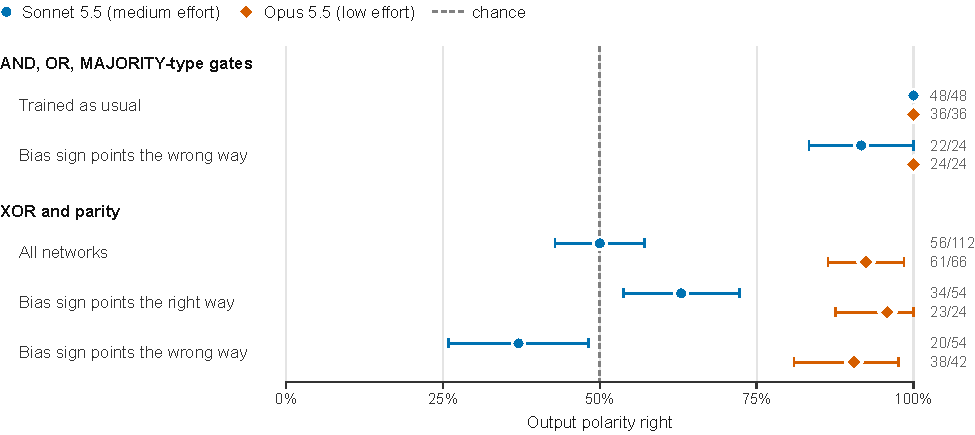
\includegraphics[width=\linewidth]{figures/fig_polarity.pdf}
\caption{Share of stimuli with output polarity (plain vs.\ NOT) right; chance is 50\%. Stimuli are single-task 2,997-weight networks shown as trained and fully negated, pooled over rounds. ``AND, OR, MAJORITY-type gates'' are the monotone gates; ``bias sign points the wrong way'' means the bias cue is reversed. Bars are 90\% bootstrap intervals over networks; counts are on the right. The split by bias-sign direction is exploratory for XOR/parity and leaves out the networks trained directly on NOT~$f$; the cue-reversed monotone networks are round~5's pre-registered test.}
\label{fig:polarity}
\end{figure}

\subsection{\Sonnet's XOR/parity answers partly follow the output bias's sign (exploratory)}
\label{sec:cue}
A natural shortcut is that a negative output bias means ``output 0 when nothing is active'', and so a plain option. That shortcut is right for \nBaseBiasMono{} of monotone stimuli but only \nBaseBiasXL{} of XOR/parity stimuli, which would explain \Sonnet's pattern.

In round~3, \Sonnet's XOR/parity polarity was right \nDOneCueRight{} times when the bias sign pointed the right way and \nDOneCueWrong{} when it pointed the wrong way (pre-registered one-sided Fisher test, $p=\nDOneCueFisher$; network-level permutation $p=\nDOneCueP$, exploratory). A pre-registered replication on 12 new networks failed: \nEOneRight{} vs.\ \nEOneWrong{}, $p=\nEOneP$. Round~4's 24 new networks, whose split by cue direction was pre-registered as a reported descriptive, show the effect again: \nSonCueFourRight{} vs.\ \nSonCueFourWrong{} (permutation $p=\nSonCueFourP$, exploratory). Pooled over all XOR/parity networks, the split is \nSonCueRight{} vs.\ \nSonCueWrong{} for \Sonnet{} (\nSonCueNets{} networks, $p=\nSonCueP$) and \nOpusCueRight{} vs.\ \nOpusCueWrong{} for \Opus{} ($p=\nOpusCueP$). Because the pre-registered replication failed and the pooled data include the round that suggested the hypothesis, we treat the effect as exploratory.

The effect is partial. Suppose \Sonnet{} follows the cue on a share $a$ of XOR/parity stimuli, follows the true polarity on a share $t$, and otherwise guesses. Then the pooled rates imply $a\approx\nSonCueFollowPct$ and $t\approx\nSonCueTruthPct$: on these gates \Sonnet{} mostly guesses. The gate matters beyond the cue. When the bias sign points the right way, \Sonnet's polarity is right on \nSonMonoCueOkPol{} monotone stimuli but on only \nSonCueRight{} XOR/parity stimuli. When it points the wrong way on monotone networks, \Sonnet{} is still right on \nRFiveSonCuePol{} (Section~\ref{sec:neg}). The shortcut is therefore specific to XOR and parity, consistent with \Sonnet{} falling back on the bias sign where it cannot work polarity out. On shared trunks \Sonnet{} shows no cue effect (polarity \nSonTrCueRight{} vs.\ \nSonTrCueWrong), but there the output bias is about eight times smaller than in single-task networks (mean $|b_2|$ \nStatTrunkRBtwo{} vs.\ \nStatSingleBtwo; Appendix~\ref{app:stats}), so the cue is less prominent.

\Sonnet's replies sometimes state the shortcut, for example: \emph{``The bias is 1.01, which is positive, so the all-zero input is likely to give output 1 unless the other contributions cancel it.''} Mention counts do not separate the two models' strategies, though. \Sonnet's XOR/parity replies mention the output bias more often than \Opus's (\nSonXLBiasMention{} vs.\ \nOpusXLBiasMention), but they also mention the all-zero input more often (\nSonXLZeroMention{} vs.\ \nOpusXLZeroMention).

\subsection{A shared first layer: \Opus{} decodes the output layer when it must choose}
\label{sec:trunk}
Each trunk is shown with four readouts, so a reader that uses only the first layer is right on at most one of them: the 25\% ceiling. On 16 rescaled trunks, \Sonnet's mean per-trunk accuracy was \nSonTrMean{} (90\% CI \nSonTrLo--\nSonTrHi\%; sign-flip test against the 25\% first-layer ceiling, $p=\nSonTrP$). \Opus's was \nOpusTrMean{} (\nOpusTrLo--\nOpusTrHi\%, $p=\nOpusTrP$). Our pre-registered rule required both upper bounds to fall below 40\% to call this ``neither decodes''. \Opus's did not, so the verdict is inconclusive for \Opus. \Sonnet{} shows no evidence of exceeding the ceiling (Figure~\ref{fig:trunks}).

\paragraph{Forced choice.} \Opus{} answered ``none of the above'' on \nOpusTrNoneR{} of these readouts. In a pre-registered follow-up we removed that option and asked for one of the 16 functions, changing nothing else. \Opus's mean per-trunk accuracy rose to \nRFiveTrMean{} (90\% CI \nRFiveTrLo--\nRFiveTrHi\%; sign-flip test against the 25\% ceiling, $p=\nRFiveTrP$): under forced choice it decodes readouts beyond what the first layer allows. On the same readouts, it was right \nRFiveTrWithQ{} times with the option and \nRFiveTrForced{} without. On the readouts it had abstained on, it was now right \nRFiveTrAbstRight{}; on the rest, \nRFiveTrRestWithQ{} became \nRFiveTrRestForced. With one sample per stimulus, the remaining gain cannot be separated from run-to-run variation, or from the prompt's implication that one option is right. \Sonnet{} was not run under forced choice.

The 25\% ceiling is the best a first-layer-only reader can do, not what it is expected to do. Such a reader gives one answer per trunk, so it expects 1/16, or 6.25\%. A reader that gets polarity right but has no information about group or gate expects 12.5\%. Against 12.5\% (exploratory), \Opus{} is above ($p=\nOpusTrPEighth$; under forced choice $p=\nRFiveTrPEighth$) and \Sonnet{} marginal ($p=\nSonTrPEighth$). Answers vary across a trunk's readouts, with at least three distinct answers in \nSonTrDistinct{} (\Sonnet) and \nOpusTrDistinct{} (\Opus) trunks. With one sample per stimulus, some of that variation may be sampling noise. The clearest evidence that answers track the readout is polarity, below. Each trunk shows a function and its negation, which share the first layer, so only the readout can separate them.

The pre-registered breakdown by level shows where the information comes from.
\begin{itemize}
\item \textbf{Input group.} \Opus{} picks the right input group above chance (\nOpusTrGrp; per-trunk sign-flip $p=\nOpusTrGrpP$, exploratory). \Sonnet{} is at chance (\nSonTrGrp). Under forced choice \Opus{} gets \nRFiveTrGrp.
\item \textbf{Pair, given the group.} Both pick the right pair more often than expected by chance (descriptive): \nSonTrPair{} and \nOpusTrPair, against about \nSonTrPairExp{} and \nOpusTrPairExp{} expected from their answer frequencies; \Opus{} under forced choice \nRFiveTrPair{} against about \nRFiveTrPairExp.
\item \textbf{Polarity, given the pair.} When they pick the right pair, they almost always get its polarity right (\nSonTrPolPair{} and \nOpusTrPolPair; \nRFiveTrPolPair{} under forced choice).
\end{itemize}
Both readers thus extract readout-specific information. Under forced choice, \Opus{} identifies about half the functions. With ``none'' allowed, neither identifies the function reliably.

The failures differ in kind. \Opus{} answered ``none of the above'' on \nOpusTrNoneR{} rescaled trunk readouts (\nOpusTrOldNone{} at the original scale), but on \nOpusSingleNone{} single-task originals. Excluding these abstentions, its exact accuracy is \nOpusTrExactAnswered. Removing the option recovers much of this loss (above). Its replies reason from the first layer: strong hidden units combine both input groups, so the function probably depends on both (\emph{``Because both groups appear to affect the output, the network most likely computes a function combining them, which is option Q''}). \Sonnet{} abstained on \nSonTrNoneR{} and exceeded its cap on \nSonTrTrunc{} (\Opus: \nOpusTrTrunc). Otherwise it named a function, mostly from the three-input group (\nSonTrThreeGroup{} of its named answers).

Rescaling did not explain the result. On the same 32 readouts, accuracy before vs.\ after rescaling was \nSonTrScale{} (\Sonnet) and \nOpusTrScale{} (\Opus). A rule that reads the input group from first-layer weight norms is right on \nBaseNormGroupSingle{} of single-task stimuli and \nBaseNormGroupTrunk{} of trunk stimuli. On trunks, the input group must therefore come from the output layer. \Opus{} recovers it above chance and \Sonnet{} does not.

\begin{figure}[t]
\centering
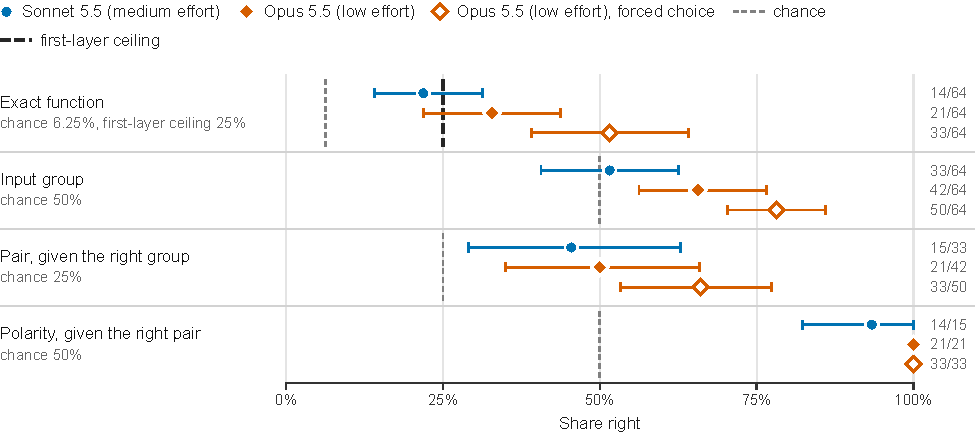
\includegraphics[width=\linewidth]{figures/fig_trunks.pdf}
\caption{Answers on shared trunks, scored at four levels: exact function, input group, pair (the function or its negation) and polarity. Trunks are rescaled to single-task weight statistics (16 trunks $\times$ 4 readouts). Dashed lines: chance, and for exact accuracy also the 25\% ceiling of a first-layer-only reader. Bars are 90\% bootstrap intervals over trunks. ``Pair'' and ``polarity'' are conditional on the previous level being right. Hollow diamonds: \Opus{} without the ``none of the above'' option (round~5).}
\label{fig:trunks}
\end{figure}

\subsection{Other settings}
\label{sec:other}
\begin{itemize}
\item \textbf{Warning prompt.} Telling \Sonnet{} that networks may have been edited in their output layer raised negation accuracy from \nWarnUnw{} to \nWarnW{} ($\nWarnGain$ points, 90\% CI $\nWarnLo$ to $\nWarnHi$), and polarity on cue-reversed stimuli from \nETwoUnw{} to \nETwoW{} ($\nETwoGain$, CI $\nETwoLo$ to $\nETwoHi$). Both results are inconclusive.
\item \textbf{\Haiku.} At low or medium effort it exceeded a 6,000-token cap on \nHaikuLowTrunc{} and \nHaikuMedTrunc{} stimuli, so it was not usable at this size.
\item \textbf{\Opus{} at low effort} exceeded its cap on \nOpusLowTrunc{} calls in rounds 3b--4.
\item \textbf{False alarms.} ``None of the above'' was given in \nNoneFASingle{} replies to intact single-task networks shown as trained (all models, rounds 3--4).
\end{itemize}

\section{Discussion}
\paragraph{What is read.} Taken together, the results suggest a reading procedure:
\begin{itemize}
\item identify the relevant inputs, and largely the gate, from the hidden units' input weights and biases, which are structured for single-task networks;
\item settle polarity from the output layer. On monotone gates a simple direction cue suffices (Section~\ref{sec:neg}). On XOR and parity it does not, but a handful of the largest terms at $x=\mathbf{0}$ decide polarity (Section~\ref{sec:xl}). One \Opus{} reply describes a case-by-case evaluation of the largest hidden units on the relevant inputs (\emph{``this comes from checking the largest units by hand''}), and \Opus's accuracy is consistent with such an evaluation, though replies need not reflect the computation. On XOR and parity, \Sonnet's answers are no better than the bias sign alone, and partly follow it (Section~\ref{sec:cue});
\item partly decode what the output layer does with shared features: polarity when the pair is right, for \Opus{} also the input group, and, under forced choice, the exact function about half the time.
\end{itemize}
This fits the debate around the game-policy result. A first layer whose input weights mirror the observation layout identifies the environment \citep{goedecke2026}, and our readers rely heavily on such first-layer structure. Concurrent work finds a similar emphasis on a network's first and last layers in small image classifiers \citep{ahmed2026memorization}. The account is also consistent with our pilot: the partial flips mostly left polarity unchanged, and \Sonnet{} missed them whether or not the network was constant.

\paragraph{Model tier.} We cannot rule out output length as an explanation of the \Opus/\Sonnet{} difference. The two wrote similar mean amounts at these settings (\nOpusMeanOut{} and \nSonMeanOut{} tokens), and \Sonnet{} given more room ran out of tokens, so we could not test whether more reasoning would help. If anything, the effort settings favour \Sonnet, which ran at medium effort and \Opus{} at low. Whether the difference reflects scale or training cannot be told from two models of one family.

\paragraph{Implications for weight auditing.} Flaws that are visible in the first layer or in polarity, such as the confounds and threshold shifts in \citet{nusrat2026auditing}, are within reach of zero-shot reading. Flaws that live in how the output layer combines shared features may not be. Shared trunks could test for this second kind.

\section{Limitations}
\begin{itemize}
\item \textbf{Scope.} We study one model family, small one-hidden-layer ReLU networks, 12 binary inputs and 16 boolean functions. Our claims are limited to this setting.
\item \textbf{Readers.} We test two Claude models from one vendor. Whether open-weight language models read weights the same way is untested; we plan to run them on the same released stimuli.
\item \textbf{Sampling and effort.} There is one sample per stimulus. \Opus{} ran at low effort and \Sonnet{} at medium, and these settings are not equivalent across models.
\item \textbf{Cue-reversed monotone networks.} Normal training almost never yields monotone networks with the bias cue reversed (\nRFiveHitsD{} and \nRFiveHitsK{} of \nRFiveSearchN{} seeds for two of six functions, none for the others). Five functions were therefore built with the output bias held positive during training or with exact function-preserving edits. These raise the largest hidden bias on three functions, and for AND and 3-AND they flip the output weights of \nRFiveFlipsLo--\nRFiveFlipsHi{} never-active units. Function and construction method are confounded. Polarity stayed right on networks without these edits as well (\nRFiveSonNoShiftPol{} for \Sonnet, \nRFiveOpusNoShiftPol{} for \Opus).
\item \textbf{Trunk statistics.} Rescaled trunks have smaller output biases than single-task networks (Appendix~\ref{app:stats}), though the biases keep their sign. Removing the ``none'' option raised \Opus's trunk accuracy (Section~\ref{sec:trunk}). \Sonnet{} was not tested under forced choice, so the two models' trunk results are not directly comparable.
\item \textbf{Fixed format.} The option order and the prompt format were fixed throughout. We see no strong preference for plain options. On XOR/parity, \Sonnet{} answered a plain option on \nSonXLAnsPlain{} stimuli, and \nSonXLLabPlain{} had plain labels. On networks trained on NOT~$f$, it answered a plain option \nNativePlain{} times. The pilot used a different, \nPilotOptions-option list.
\item \textbf{Adaptive rounds.} Rounds 3b--5 were added after seeing results. The bias-sign effect is exploratory, because its pre-registered replication failed. Pre-registration timestamps are self-reported for every round except round~4.
\item \textbf{Model change.} Closed models change over time. We report model identifiers and call dates (November 2026) and release every reply.
\end{itemize}

\section{Conclusion}
Exact weight edits that keep or invert a network's function show where zero-shot weight reading by two Claude models stops for small MLPs. Both lean on the first layer's structure, and on monotone gates both take output polarity from the output layer, even when the output bias's sign points the wrong way. On XOR and parity, where a simple direction cue fails, \Opus{} still gets polarity right, while \Sonnet{} mostly guesses, partly from the bias sign (exploratory). On a shared first layer, both extract some readout-specific information. When it must choose, \Opus{} identifies about half the functions, well above what the first layer allows, but neither model identifies them reliably. Running open-weight readers on the same stimuli is the natural next step. Before the results of a function-breaking control are interpreted, it should be checked for degeneracy and for whether it changes what a reader using only coarse cues can see.

\section*{Broader impact statement}
Using language models to audit model weights could help safety review, but for two models and small networks we find output-layer reading only partial. We caution against treating zero-shot weight reading as certification.

\section*{Reproducibility statement}
Code to generate every stimulus (with seeds), the exact prompts, all \nRFiveTotalCalls{} API replies with token counts and model identifiers, the pre-registration files with hashes, and the script that produces every number and figure in this paper (\texttt{analysis.py}, which writes the macros used in this text) \codelink.

\section*{Use of AI assistants}
An AI coding assistant (Claude Code) was used to write the experiment code, run the experiments, compute the analyses and draft text, under the author's direction and review. The models under study come from the same vendor as the assistant. All numbers in the paper are generated by code from the saved replies. The author takes full responsibility for the content.

\bibliography{references}
\bibliographystyle{tmlr}

\appendix
\section{Prompt}
\label{app:prompt}
The full prompt for a 505-weight network, with most weight lines elided, is below. The system prompt was ``You are a careful analyst. Answer the question about the network you are given.''
\begin{lstlisting}
The network below is an MLP with 12 binary inputs x0..x11 (each 0 or 1), one ReLU hidden layer, and one output logit (output = 1 if logit > 0, else 0). Decide which boolean function it computes over all 4096 inputs. Options (same for every network):
A: output = x2 AND x5
B: output = x2 OR x5
C: output = x2 XOR x5
D: output = x2 AND (NOT x5)
E: output = NOT (x2 AND x5)
F: output = NOT (x2 OR x5)
G: output = NOT (x2 XOR x5)
H: output = NOT (x2 AND (NOT x5))
I: output = MAJORITY(x0, x3, x7)
J: output = x0 AND x3 AND x7
K: output = x0 OR x3 OR x7
L: output = PARITY(x0, x3, x7)  (1 if an odd number are 1)
M: output = NOT MAJORITY(x0, x3, x7)
N: output = NOT (x0 AND x3 AND x7)
O: output = NOT (x0 OR x3 OR x7)
P: output = NOT PARITY(x0, x3, x7)  (1 if an even number are 1)
Q: none of the above (the network computes some other function)

Any option may be correct, including Q. Note that several options share the same inputs, so knowing which inputs matter is not enough.

### Network (505 weights)
Layer 1 (input 12 -> hidden 36, ReLU). Row j = hidden unit j: its 12 input weights for x0..x11, then its bias.
h0: 1.05 -0.0932 -0.183 0.651 -0.0736 0.0158 0.129 1.07 0.0768 -0.0184 -0.0447 0.0638 | bias -0.523
...
Layer 2 (hidden 36 -> 1 output logit; output 1 if logit > 0). Weights for h0..h35 in order, then bias.
out: 0.632 1.3 -1.15 -0.532 ... | bias ...

Work it out from the weights. Do not write or run code. End your reply with one final line exactly in this form: ANSWER: <one letter from A to Q>
\end{lstlisting}
The warning used in the warning condition was inserted after the sentence beginning ``Note that'': ``Caution: some networks were edited after training, for example in their output layer, so the first layer alone may not tell you the function. Check how the output layer combines the hidden units before you answer.''

\section{Weight statistics}
\label{app:stats}
\begin{table}[h]
\centering\small
\caption{Mean absolute values of the displayed weights at 2,997 weights.}
\begin{tabular}{@{}lcccc@{}}
\toprule
Networks & $|W_1|$ & $|b_1|$ & $|W_2|$ & $|b_2|$ \\
\midrule
Single-task, all gates (original) & \nStatSingleWone & \nStatSingleBone & \nStatSingleWtwo & \nStatSingleBtwo \\
Shared trunks, as trained & \nStatTrunkWone & \nStatTrunkBone & \nStatTrunkWtwo & \nStatTrunkBtwo \\
Shared trunks, rescaled & \nStatTrunkRWone & \nStatTrunkRBone & \nStatTrunkRWtwo & \nStatTrunkRBtwo \\
Single-task, monotone gates only &\nRFiveStatNegMonoWone & \nRFiveStatNegMonoBone & \nRFiveStatNegMonoWtwo & \nRFiveStatNegMonoBtwo \\
Monotone, cue reversed (round~5) & \nRFiveStatCueWone & \nRFiveStatCueBone & \nRFiveStatCueWtwo & \nRFiveStatCueBtwo \\
\bottomrule
\end{tabular}
\end{table}

\clearpage
\section{All decision rules}
\label{app:rules}
Table~\ref{tab:rules} lists every pre-registered decision rule.

\begin{table}[h]
\centering\small
\caption{Every pre-registered decision rule, in the order of the rounds. ``Inconclusive'' means the pre-registered thresholds were met in neither direction. Verdicts use the wording of the plans. Omitted IDs (D4, D6, E3, F4b) are descriptive analyses.}
\label{tab:rules}
\begin{tabular}{@{}lp{5.3cm}l@{}}
\toprule
Rule & Result & Verdict \\
\midrule
Pilot gate (\Sonnet) & \nPilotOrig{} vs.\ \nPilotCaught, $p=\nPilotP$; rule committed after its calls & go; reinterpreted (Section~\ref{sec:dead}) \\
D1, polarity under negation (\Sonnet) & sensitivity \nDOneS{} points, CI \nDOneLo{} to \nDOneHi{} & reads polarity \\
D1-cue, bias-cue split (\Sonnet, descriptive) & \nDOneCueRight{} vs.\ \nDOneCueWrong, Fisher $p=\nDOneCueFisher$ & bias-sign shortcut \\
D2, trunks, original scale (\Sonnet) & \nSonTrOldExact{} exact & no evidence of decoding \\
D3, warning (\Sonnet) & \nWarnUnw{} $\to$ \nWarnW{}, CI $\nWarnLo$ to $\nWarnHi$ & inconclusive \\
D5, \Haiku{} & \nHaikuLowTrunc{} and \nHaikuMedTrunc{} truncated & not usable \\
E1, bias-cue replication & \nEOneRight{} vs.\ \nEOneWrong, $p=\nEOneP$ & not replicated \\
E2, warning on cue-reversed stimuli & \nETwoUnw{} $\to$ \nETwoW{}, CI $\nETwoLo$ to $\nETwoHi$ & inconclusive \\
E4, trunks, original scale (\Opus) & \nOpusTrOldExact{} exact & no evidence of decoding \\
F3, \Opus{} vs.\ \Sonnet{} on XOR/parity & \nFThreeOpus{} vs.\ \nFThreeSon, $p=\nFThreeP$ & replicated \\
F4a, rescaled trunks & \Sonnet{} \nSonTrMean{} [\nSonTrLo, \nSonTrHi]; \Opus{} \nOpusTrMean{} [\nOpusTrLo, \nOpusTrHi] & inconclusive \\
G1, cue-reversed monotone (\Sonnet) & \nRFiveSonCuePol{} vs.\ \nRFiveSonBasePol, Fisher $p=\nRFiveSonFisherP$ & computes polarity \\
G2, cue-reversed monotone (\Opus) & \nRFiveOpusCuePol{} vs.\ \nRFiveOpusBasePol & computes polarity \\
G3, trunks, forced choice (\Opus) & \nRFiveTrMean{} [\nRFiveTrLo, \nRFiveTrHi], $p=\nRFiveTrP$ & decodes \\
\bottomrule
\end{tabular}
\end{table}

Some descriptive analyses in the text were also listed in the pre-registration files as descriptive: the round-3 bias-cue split, native NOT networks, 505-weight networks, \Opus{} at medium effort, and \Sonnet{} at high effort. So were the trunk breakdown by level, the distinct answers per trunk (in round~3), and, in round~4, the split by bias-cue direction. In round~5, the split by version and function, the network-level permutation test and the 12.5\% baseline under forced choice were pre-registered as reported, as was the comparison of the same readouts with and without the ``none'' option. Others were not pre-registered: the pooled bias-cue analysis and the cue-following estimate, significance tests on round~4's cue split and on the trunk input group, the 12.5\% trunk baseline in round~4, the abstentions on trunks, the reply-text counts, the gate errors on networks with flipped never-active units, and the offline baselines.

\end{document}
